\tikzstyle{every node}=[draw=black,thick]
\tikzstyle{red}=[draw=red,color=red,thick]
\tikzstyle{black}=[draw=black,color=black,thick]
\begin{center}
    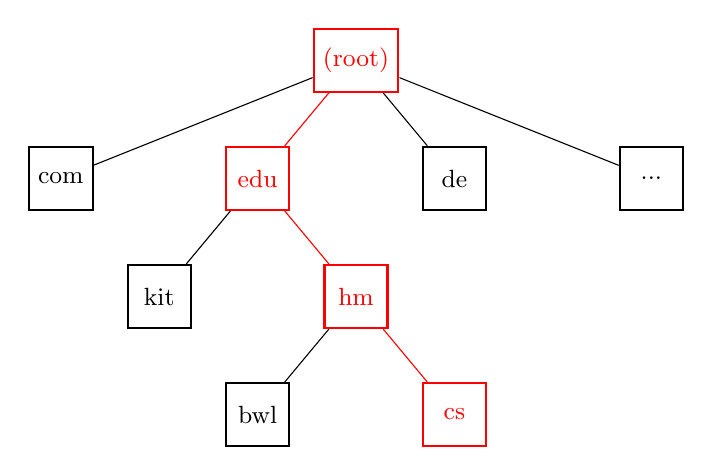
\begin{tikzpicture}
    [font=\small, edge from parent, 
    every node/.style={rectangle, minimum size=8mm, draw=black, thick, align=center},
    level distance=1.5cm,
    sibling distance=2.5cm
    ]
    \node [red] {(root)}
        child {node {com}}
        child {node [red] {edu} edge from parent[draw=red]{}       
            child {node {kit} edge from parent[draw=black]{}}
            child {node [red] {hm} edge from parent[draw=red]{}        
                child {node {bwl} edge from parent[draw=black]{}}
                child {node [red] {cs} edge from parent[draw=red]{}}
            }                
        }
        child {node {de}}
        child {node {...}};
    \end{tikzpicture}
\end{center}